\documentclass[12pt, a4paper]{article}
\usepackage[UTF8]{ctex}
\usepackage{amsmath}
\usepackage{amssymb}
\usepackage{amsthm}
\usepackage{geometry}
\usepackage{enumitem}
\usepackage{indentfirst}
\usepackage{caption}
\usepackage{fancyhdr}
\usepackage{booktabs}
\usepackage{titlesec}
\usepackage{draftwatermark}%水印
\usepackage{graphicx} % 导入图像的宏包、单图
% 页面布局设置
\geometry{top=2.54cm, bottom=2.54cm, left=3.18cm, right=3.18cm}

\SetWatermarkText{B站：布加拉提}
\SetWatermarkScale{0.4}

% 行距设置
\linespread{1.5}

% 段落设置
\setlength{\parindent}{2em}
\setlength{\parskip}{0.5em}

% 节标题格式设置
\titleformat{\section}{\normalfont\Large\bfseries}{第\chinese{section}章、}{1em}{}
\titlespacing{\section}{0pt}{2.5ex plus 1ex minus .2ex}{1.3ex plus .2ex}

% 定理环境设置
\newtheoremstyle{solution}
{}
{}
{}
{}
{\bfseries}
{、}
{1em}
{}
\theoremstyle{solution}
\newtheorem{sol}{解}

% 页眉页脚设置
\pagestyle{fancy}
\fancyhf{}
\fancyhead[C]{b站布加拉提整理（回忆版）b站甘茶w独家讲解}
\fancyfoot[C]{\thepage}

\rfoot{整理人：八方\\资源提供：考研乔瑟夫}
\lhead{
\includegraphics[width=0.06\linewidth]{p1.png}}
\rhead{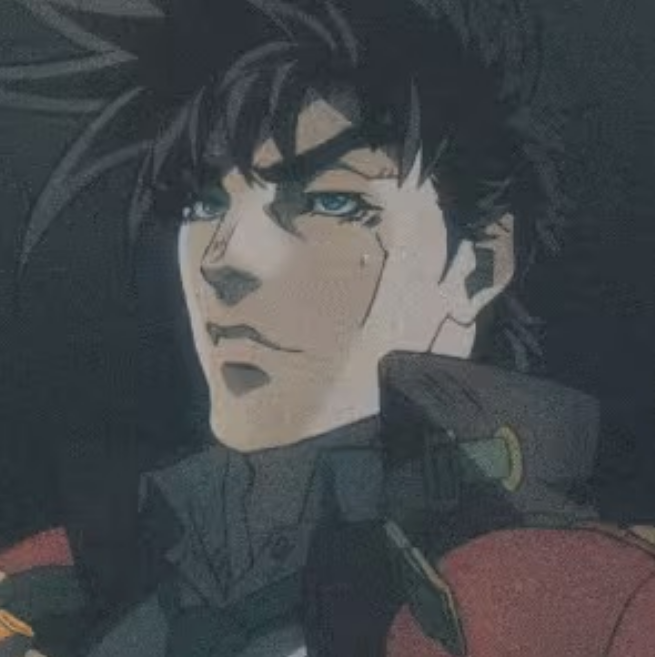
\includegraphics[width=0.06\linewidth]{p2.png}}
\renewcommand{\headrulewidth}{0.4pt}
\renewcommand{\footrulewidth}{0.4pt}

\begin{document}

\begin{center}
\Large\textbf{2019哈工大硕士考试试题：805物理光学}
\end{center}





\section*{一、填空题（20分）}
\begin{enumerate}
    \item 光的偏振态有\_\_\_\_\_，\_\_\_\_\_，\_\_\_\_\_，线偏振光\_\_\_\_\_。
    \item 单色光从水到空气，光的\_\_\_\_\_不变，\_\_\_\_\_变大。
    \item 表征干涉程度的物理量叫做\_\_\_\_\_，它的定义是\_\_\_\_\_。
    \item （重复）将一工件放入干涉光路中形成劈尖，观察到干涉条纹有弯曲，相邻暗纹间距为$e$，条纹最大弯曲度处与该条纹的间距为$0.8e$，若光波波长为$\lambda$,那么不平处的高度为\_\_\_\_\_，如果工件有凹陷，条纹弯曲的方向是\_\_\_\_\_劈尖。
    \item 使自然光变为偏振光的器件叫做\_\_\_\_\_，检验偏振光的器件叫做\_\_\_\_\_。
    \item （重复）一个线偏振光在玻璃中传播时的表达式为：$E_x=0,E_y=0,E_z=(100V/m)(\pi\times10^{14}\times s^{-1}(t-\frac{x}{c})+\frac{\pi}{2})$,求该光的频率，波长，振幅，周期，初相位是多少？（简答改填空）
    \item 根据瑞利判据，望远镜的分辨率为\_\_\_\_\_，照相机物镜的分辨率为\_\_\_\_\_，显微镜的分辨率为\_\_\_\_\_。
\end{enumerate}
\section*{二、选择题（21分）}
\begin{enumerate}
    \item 在双缝干涉实验中，两缝宽度相等，若其中一个缝的宽度略微变窄，则\_\_\_\_\_。
    A.干涉条纹的间距变宽 \quad B.干涉条纹的间距变窄 \quad C.干涉条纹的间距不变，但原来极小处的强度不在为0 \quad D.不再发生干涉
    \item 一束光强为$I_0$的线偏振光通过两个偏振片$P_1,P_2$，$P_1,P_2$的偏振方向与原入射光的光矢量振动方向的夹角分别是 $\alpha$和90度。则通过两偏振片后的光强是\_\_\_\_\_。
    A.$\frac{1}{2}I_0cos2\alpha$ \quad B.$\frac{1}{4}I_0cos2(2\alpha)$\quad C.$\frac{1}{4}I_0sin2\alpha$\quad D.$I_0cos4\alpha$
    \item 单色平行光垂直照射在光学薄膜上，经上下两个表面反射的两束光发生干涉，若薄膜的厚度为 $h$，$n_1,n_2,n_3$相应为入射介质，薄膜和基底材料的折射率，且 $n_1>n_2>n_3$  ，$\lambda$为入射光在$n_2$，中的波长，则两束反射光的光程差为\_\_\_\_\_.
    A.$2n_2h-\lambda/2$ \quad B.$2n_2h-n_2\lambda/2$ \quad C.$2n_2h$ \quad D.$2n_2h-n_1\lambda/2$ \quad
    \item 在迈克尔逊干涉仪的一条光路中，垂直光线放入折射率为$n$，厚度为$h$的透明介质片，放入后，两光程差的改变量为\_\_\_\_\_。
    A.$2(n-1)h$ \quad B.$2nh$ \quad C.$nh$ \quad D.$(n-1)h$
    \item 观察单缝弗朗合费衍射图样时，单缝宽度增加，屏上中央亮纹宽度\_\_\_\_\_。
    A.不变 \quad B.变小\quad C.变大\quad D.不变\quad
    \item 能流密度矢量S与电场强度E和磁场强度H的关系是\_\_\_\_\_。
    A.S与E，H成正比\quad B.S与E，H1成反比\quad C.$\overrightarrow{S}$与$\overrightarrow{ H},\overrightarrow{ E}$ 成正比\quad D.$\overrightarrow{S}$与$\overrightarrow{ H},\overrightarrow{ E}$成反比
\end{enumerate}
\section*{三、名词解释（28分）}
\begin{enumerate}
    \item 光源的临界宽度
    \item 主平面和主截面
    \item 瑞利判据
    \item 法拉第效应    
    \item 1/4波片
    \item 半波损失
    \item 艾里斑
\end{enumerate}
\section*{四、简答题（30分）}
\begin{enumerate}
    \item 通过偏振片观察部分偏振光时，当偏振片绕入射光方向转到某位置上，透射光强为极大，然后再将偏振片旋转30度，发现透射光强为极大值的4/5，求该入射偏振光的偏振度P及该光的自然光与偏振光光强之比。
    \item 双星之间的角距离为$1\times10^{-6}rad$，其辐射波长为$577nm,579nm$两个波长。问：
          \begin{enumerate}
            \item 望远镜的口径需要多大才能分辨此双星的像
            \item 若要用一级谱线分辨两波长，光栅条数应为多少？
          \end{enumerate}
\end{enumerate}
\section*{六、论述题（10分）}
\begin{enumerate}
    \item 实验室购进一种细丝，设计实验测出细丝直径，简述原理并画出示意图。
\end{enumerate}
\end{document}